\chapter{Implementation, Integration, and Test Plan}
In this section it's presented the order of the implementation of subsystems and its components: moreover, also a plan of the integration and test of the integration will be presented.\\
Subsystems are developed and integrated following a bottom-up approach: this choice is due to the fact that individual parts of the system are specified in detail and all parts are linked to form larger components which are in turn linked until a complete system is formed. In this way can be made decisions about reusable low-level utilities and then decide how there will be put together to create high-level construct.\\
Important to note is that both client infrastructure and server infrastructure are developed and tested simultaneously and incrementally, thanks to their independency.
\section{Implementation plan}
As said before, the implementation of the system is realised following a bottom-up method with continuous intermediate releases: obviously the attention is focused on server-side implementation because the client-side uses only APIs and functionalities that server provides.\\
Specifically:
\begin{itemize}
    \item \textbf{DBMS and DataManager}: this is the first part to implement. It incorporates all the eMall system data and allows to access to all the system data.
    \item \textbf{Authentication and AuthHandler}: authentication module is necessary at this point to provide privileges and authorizations to all kind of users of the system.
    \item \textbf{MailManager, DSOManager, PaymentManager}: external APIs module that are developed in parallel because they are each other independent.
    \item \textbf{ScanHandler, StatusHandler, eMSPHandler, CPMSHandler}: developed in parallel but after the development of the manager components of the point above.
    \item \textbf{End user app, CMPS app, Charging Socket Scan}: in the end of the whole process, it's time to implement all the client application that are responsible of UI.
\end{itemize}
\section{Integration and Test Plan}
\subsection{Integration steps}
The following images represent the integration steps for the eMall system: they provide a visual organization of the layered architecture developed.
\begin{figure}[H]
    \centering
    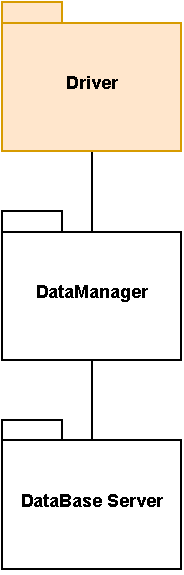
\includegraphics[width=0.2\textwidth]{images/1.pdf}
    \caption{First level of integration}
    \label{fig:1}
\end{figure}
\begin{figure}[H]
    \centering
    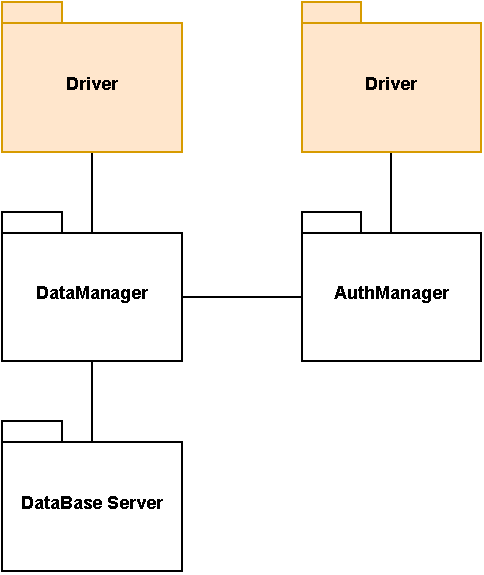
\includegraphics[width=0.4\textwidth]{images/2.pdf}
    \caption{Second level of integration}
    \label{fig:1}
\end{figure}
\begin{figure}[H]
    \centering
    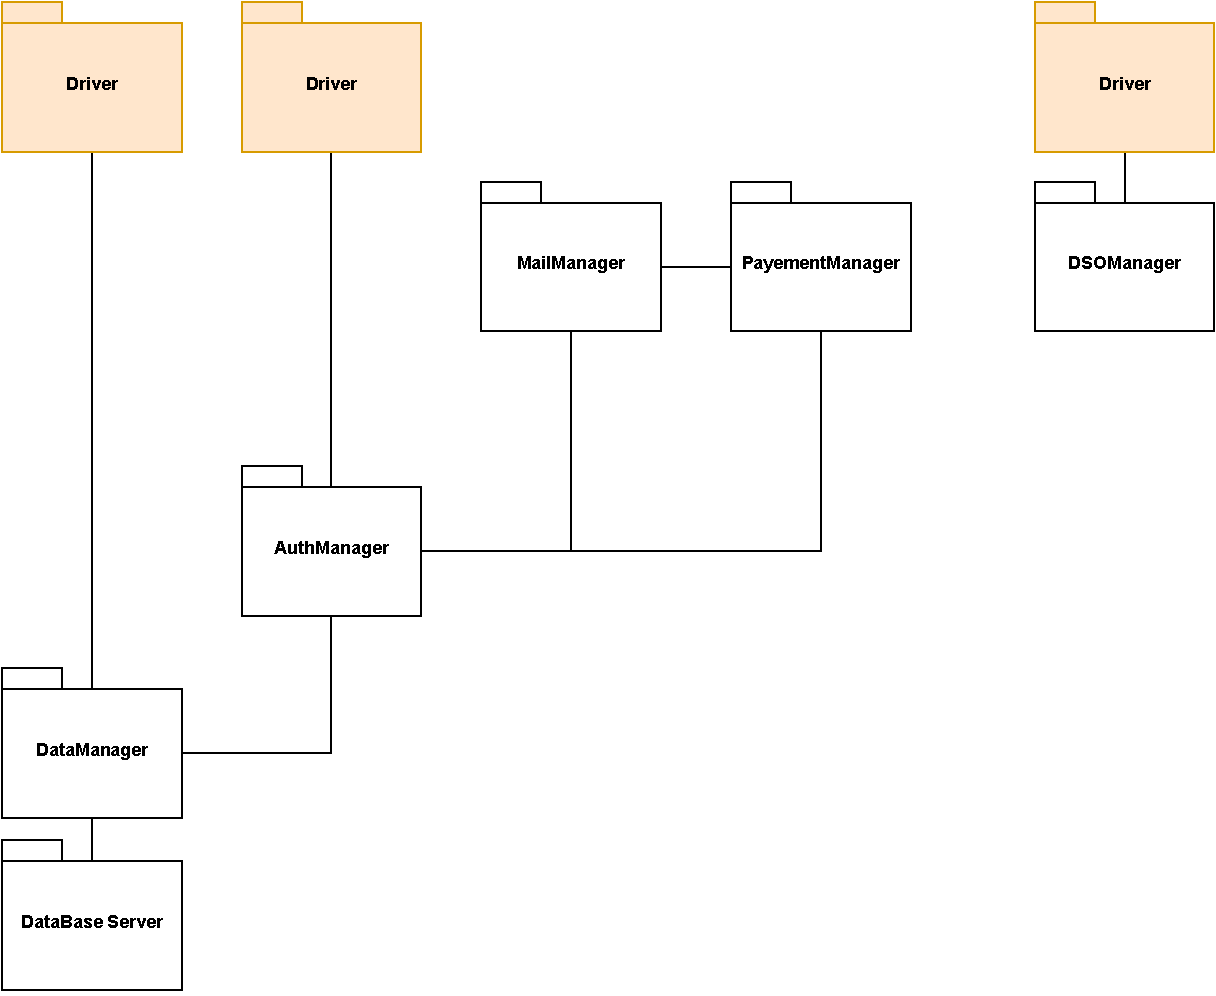
\includegraphics[width=\textwidth]{images/3.pdf}
    \caption{Third level of integration}
    \label{fig:1}
\end{figure}
\begin{figure}[H]
    \centering
    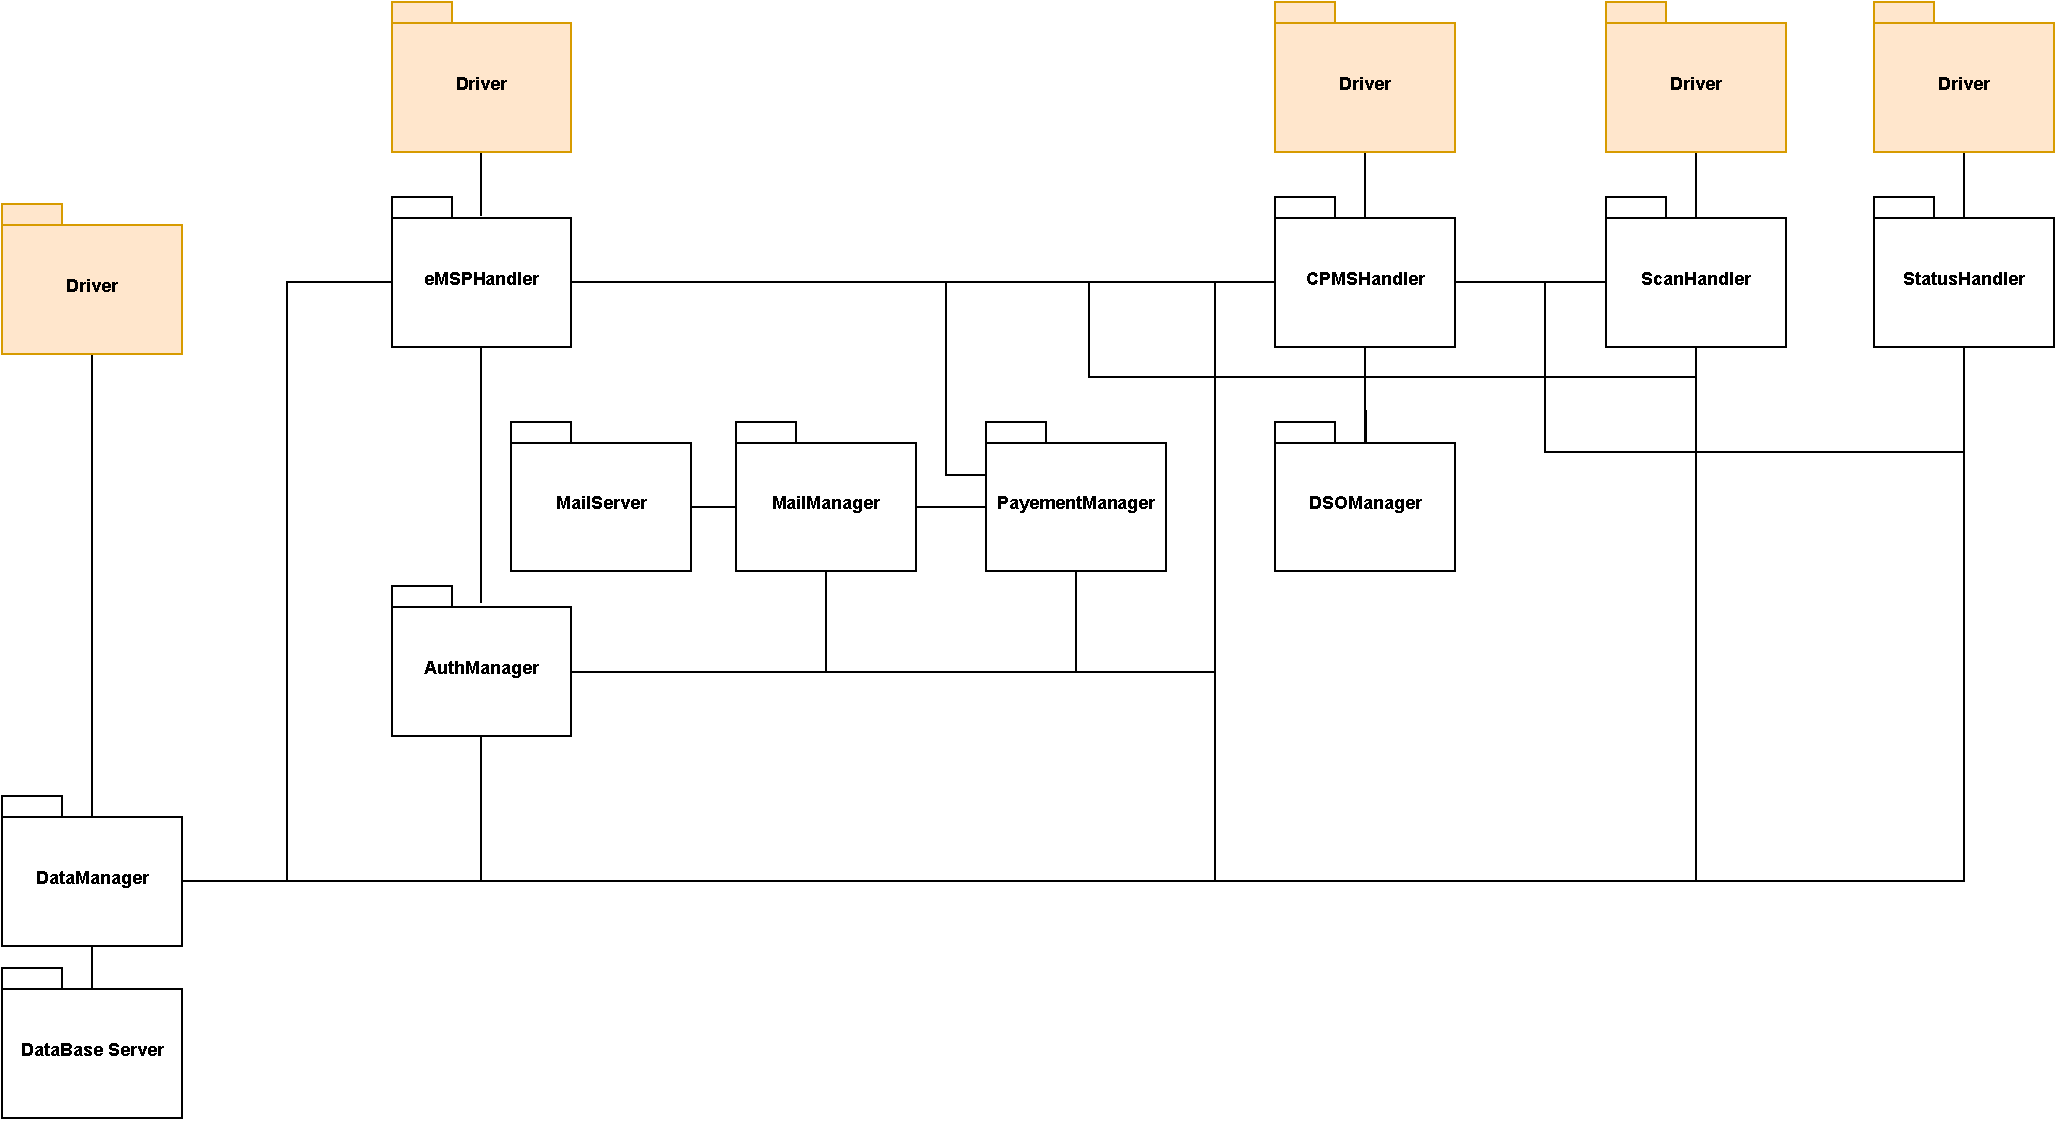
\includegraphics[width=\textwidth]{images/4.pdf}
    \caption{Fourth level of integration}
    \label{fig:1}
\end{figure}
\begin{figure}[H]
    \centering
    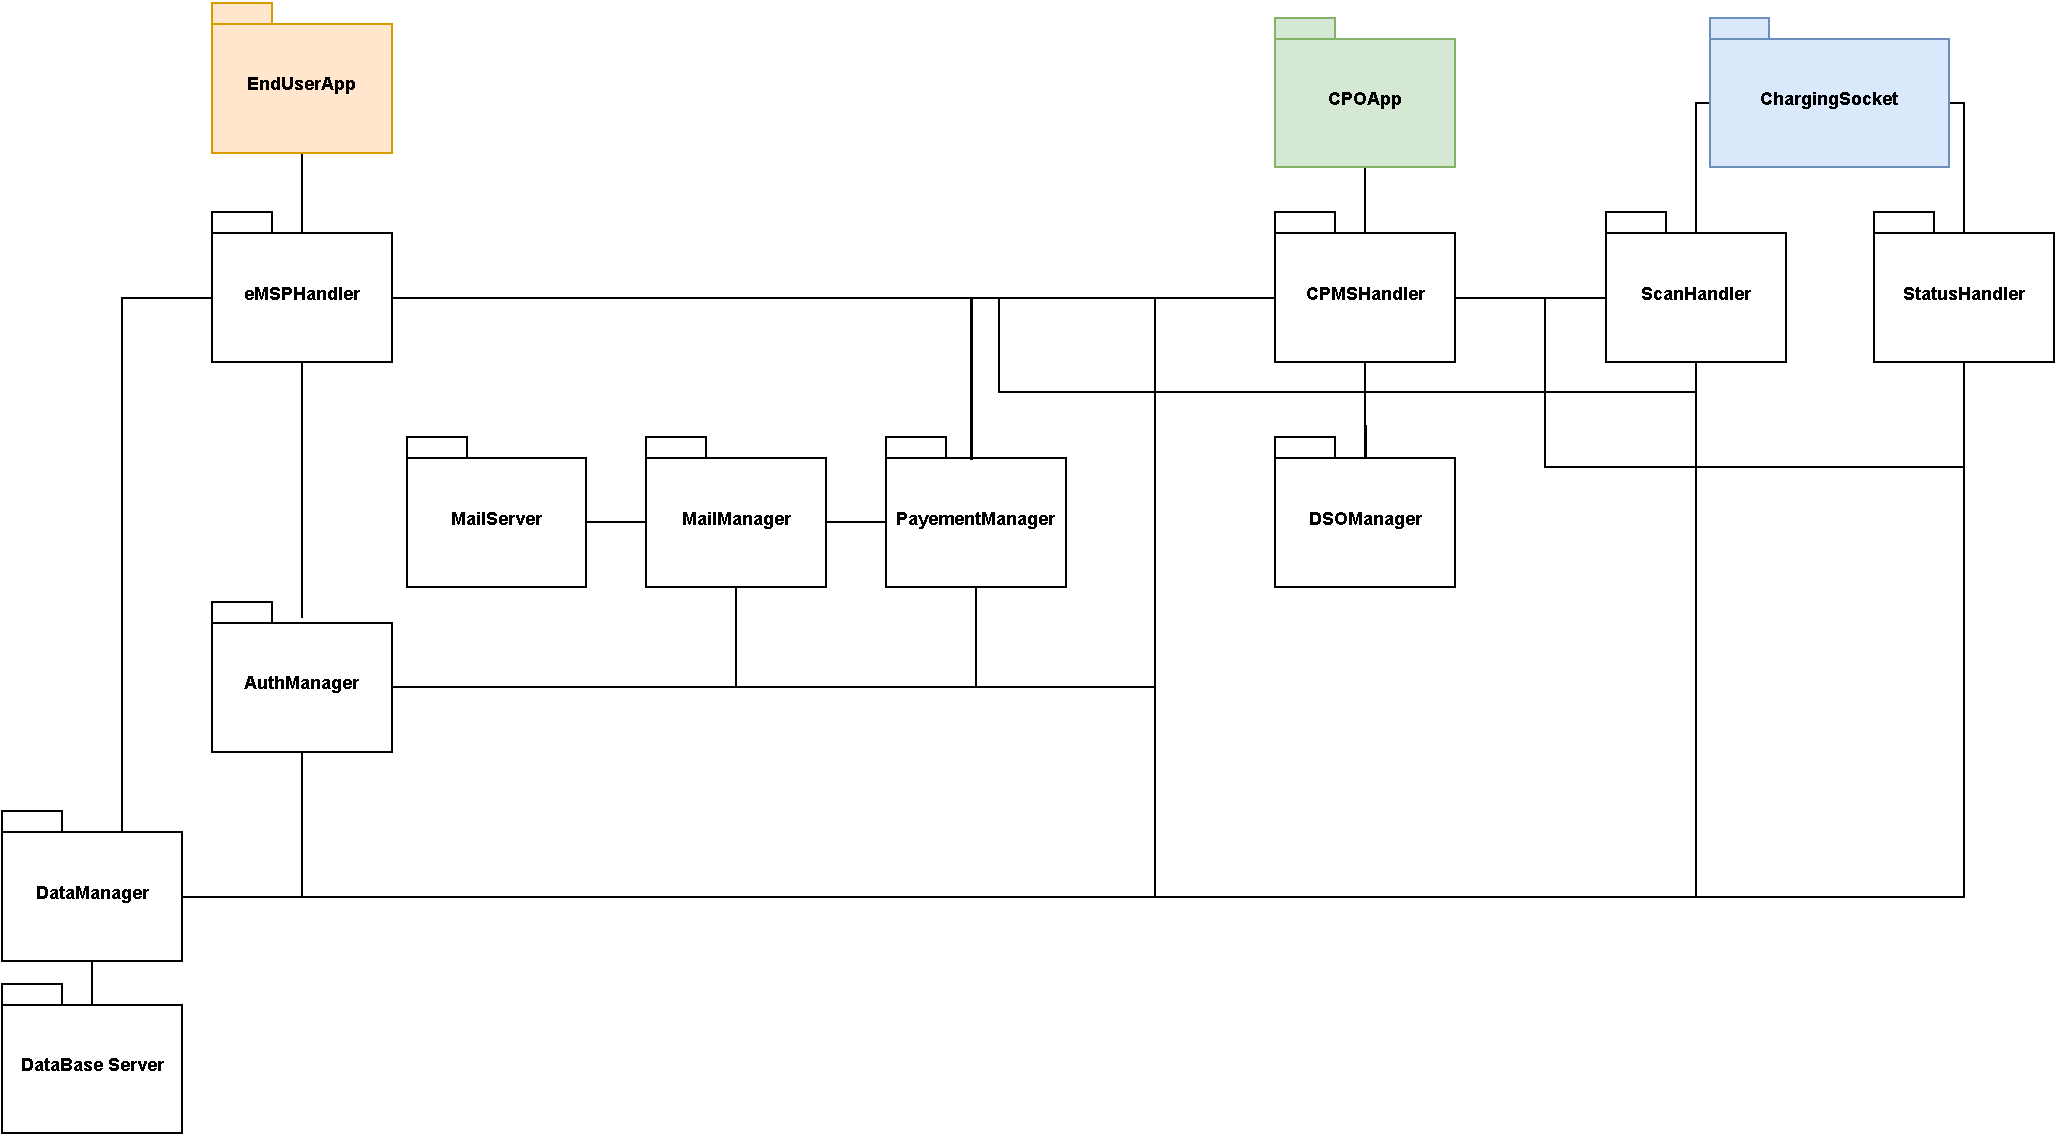
\includegraphics[width=\textwidth]{images/5.pdf}
    \caption{Fifth level of integration}
    \label{fig:1}
\end{figure}
\subsection{Testing}
During and after the developping of the eMall system, a meticulous testing phase can start to ensure that all requiremets are met.
Indeed, some components can be developed in parallel and this behaviour allows to perform some testing during the implementation phase enabling intermediate releases.\\
Obviously, when the system is ready to be released a full testing phase can be performed on the whole system. 